\documentclass{../cssheet}

%--------------------------------------------------------------------------------------------------------------
% Basic meta data
%--------------------------------------------------------------------------------------------------------------

\title{Die Satzgruppe des Pythagoras}
\author{Prof. Dr. Christian Spannagel}
\date{\today}
\setsubject{Aufgabenblatt Geometrie}
\setkeywords{geometrie}
\setpdfmetadata


%--------------------------------------------------------------------------------------------------------------
% document
%--------------------------------------------------------------------------------------------------------------

\begin{document}
\printtitle

\textbf{Aufgabe 1 (Binomische Formeln):}  Beweist die drei binomischen Formeln mit Hilfe einer geeigneten Zeichnung!

\textbf{Aufgabe 2 (Satz des Pythagoras):}  Wie lautet der Satz des Pythagoras? Formuliert ihn aus!

\textbf{Aufgabe 3 (Beweis 1):}  Führt einen Beweis des Satzes des Pythagoras mit Hilfe des folgenden Bildes durch! Wie hängt dieser Beweis mit Aufgabe~1 zusammen?
\begin{center}
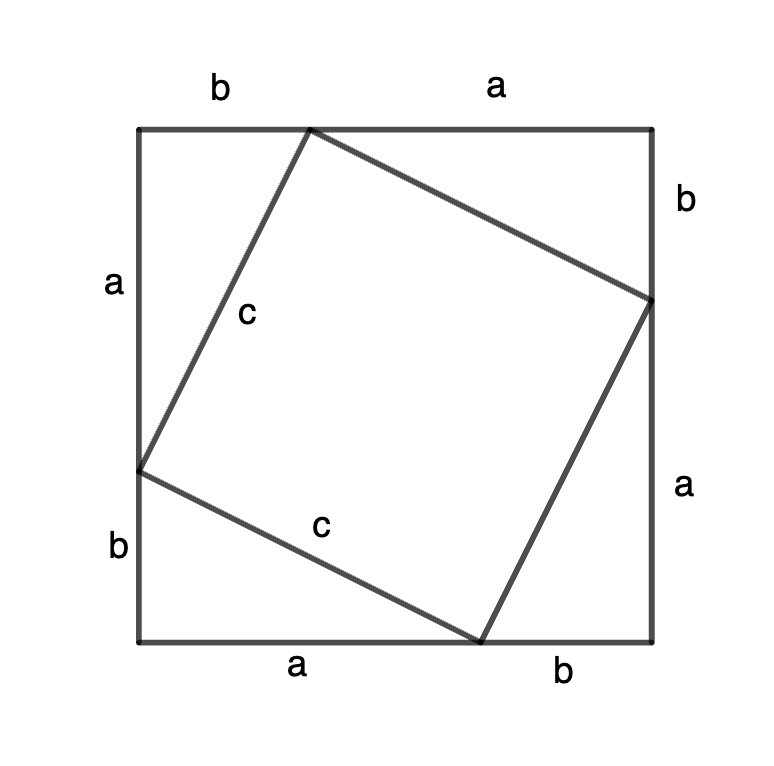
\includegraphics[width=8cm]{satz-des-py-01.png}
\end{center}

\textbf{Aufgabe 4 (Beweis 2):}  Führt einen Beweis des Satzes des Pythagoras mit Hilfe des folgenden Bildes durch!
\begin{center}
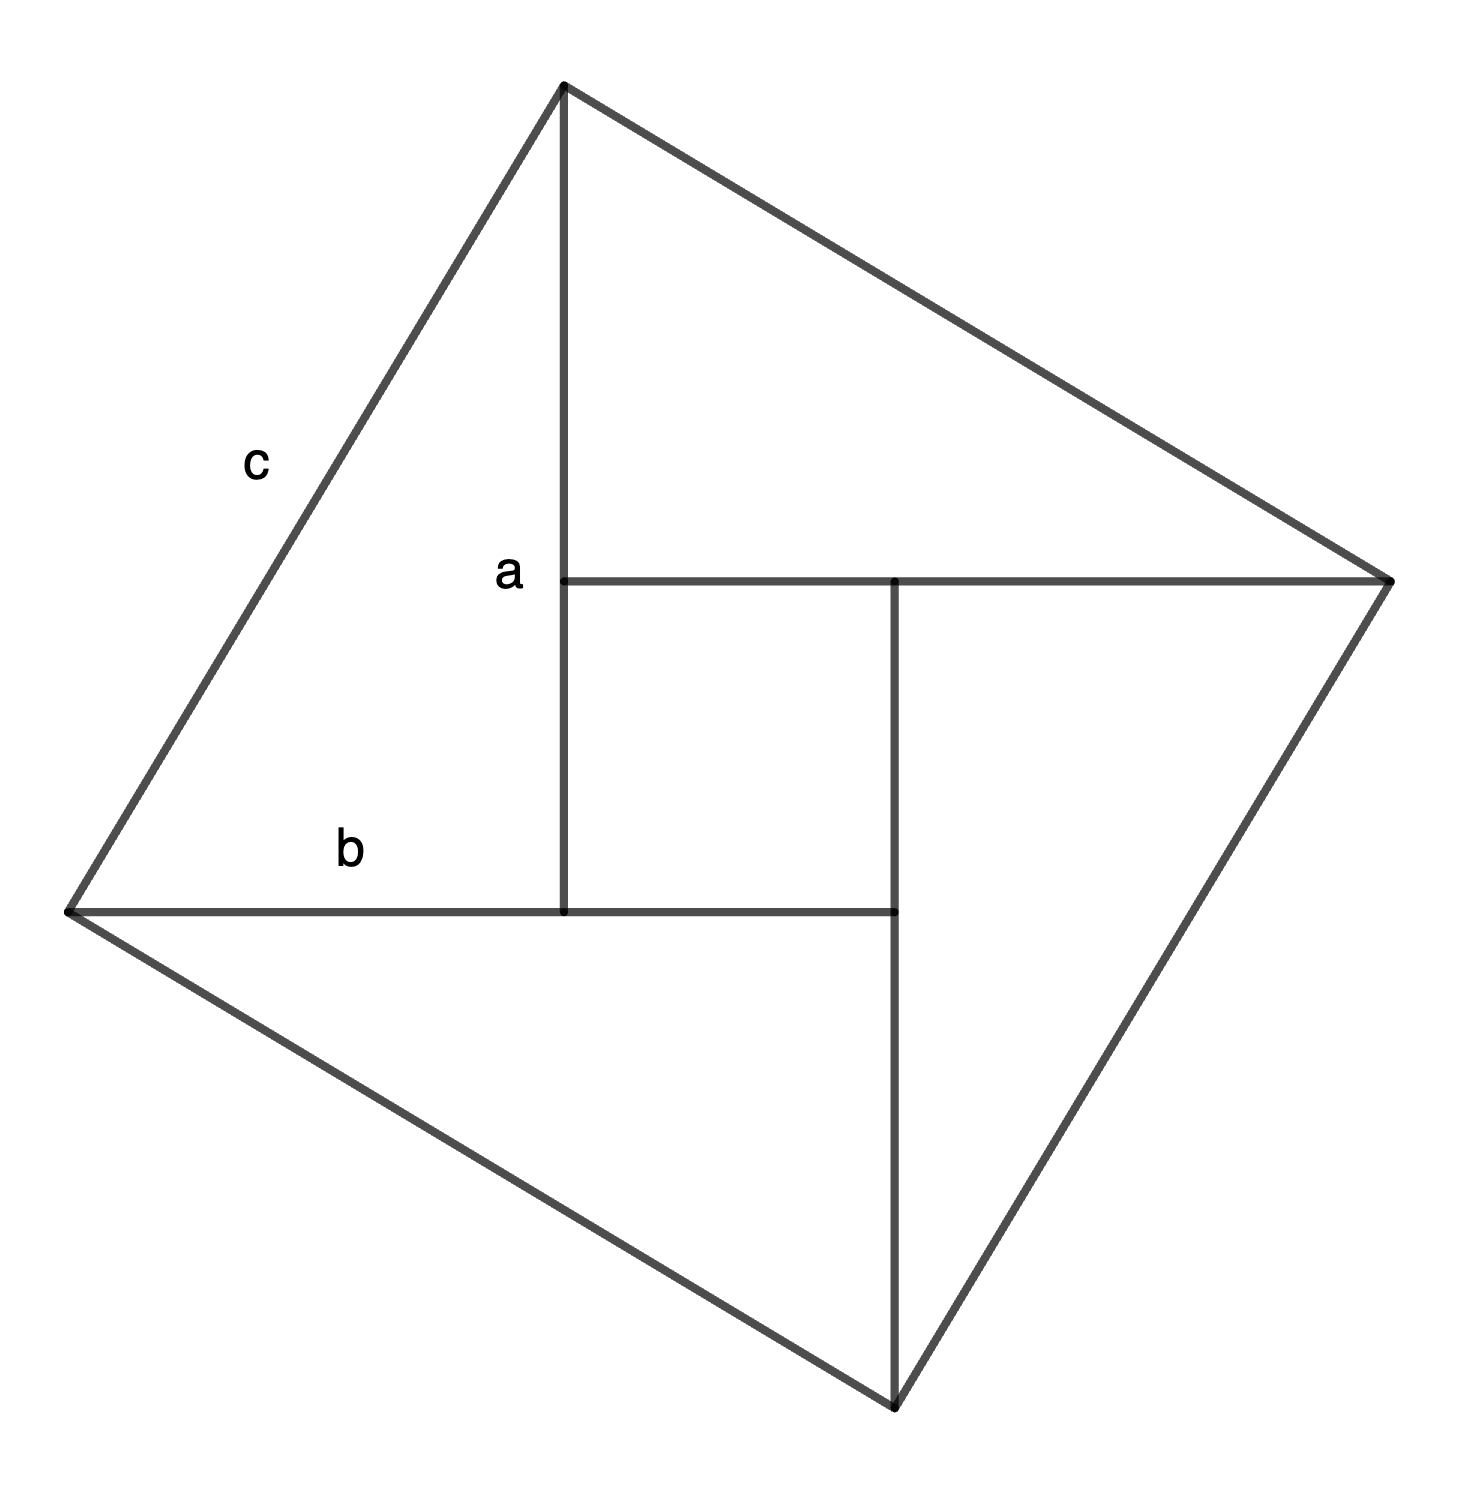
\includegraphics[width=8cm]{satz-des-py-02.png}
\end{center}
\textbf{Aufgabe 5 (Höhensatz):} Betrachtet das folgende Bild.
\begin{center}
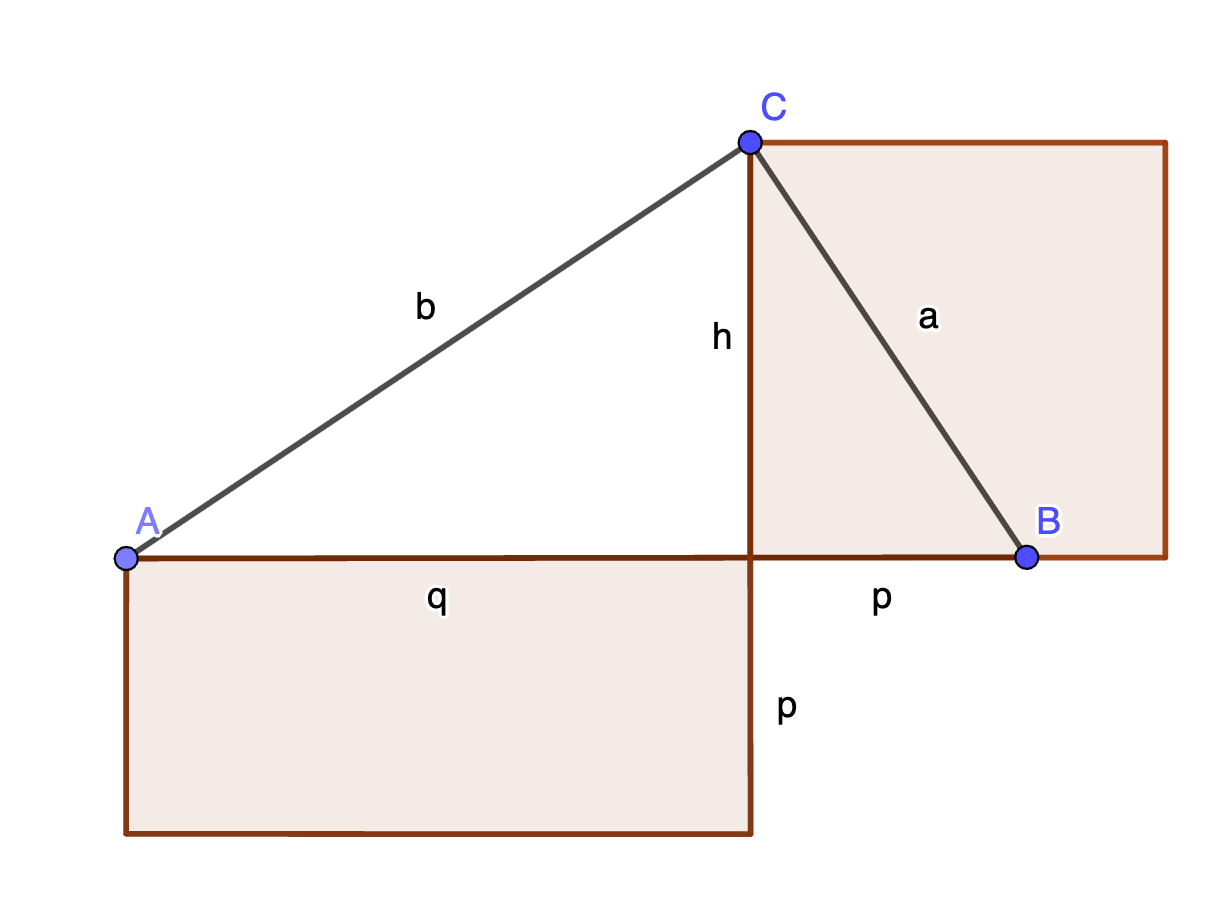
\includegraphics[width=8cm]{hoehensatz.png}
\end{center}
Der Höhensatz des Euklid besagt für rechtwinklige Dreiecke: $h^2=p\cdot q$.
Formuliert den Höhensatz sprachlich, und dann beweist den Höhensatz! Tipp: Ihr könnt dreimal den Satz des Pythagoras verwenden, und außerdem ist die erste binomische Formel hilfreich.
%\newpage

\textbf{Aufgabe 6 (Kathetensatz):} Betrachtet das folgende Bild.
\begin{center}
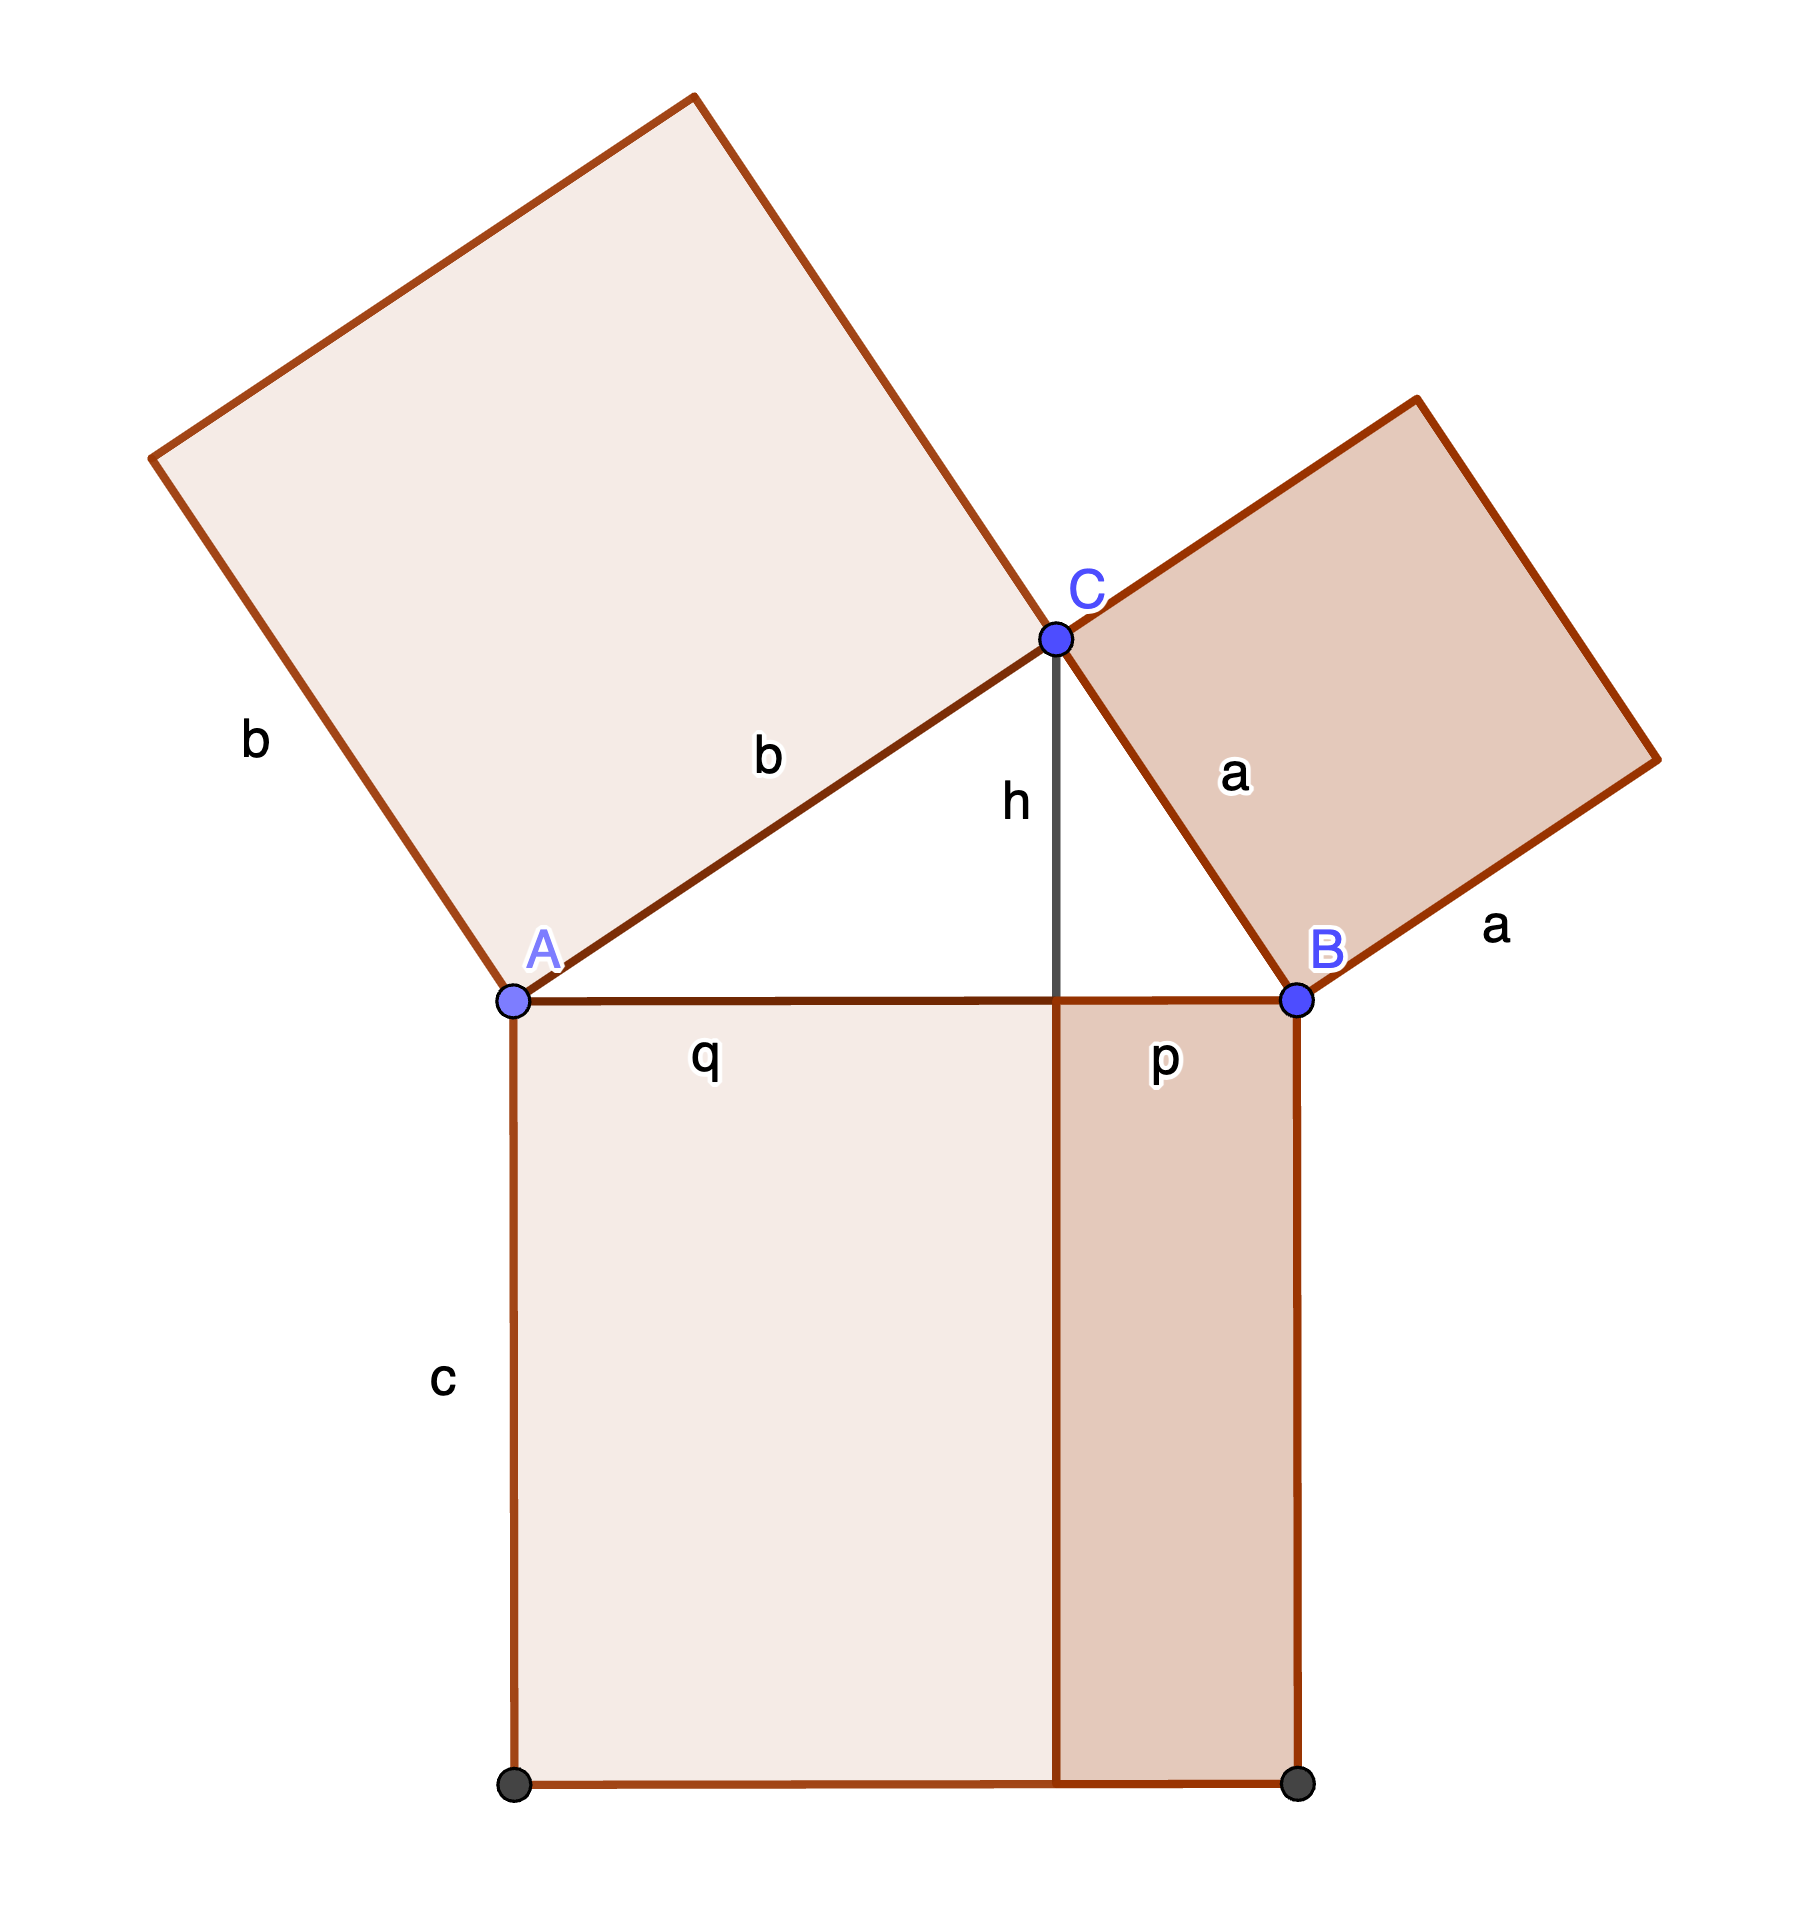
\includegraphics[width=8cm]{kathetensatz.png}
\end{center}

Der Kathetensatz für rechtwinklige Dreiecke besagt: $a^2=p\cdot c$ und $b^2=q\cdot c$. Formuliert den Kathetensatz sprachlich, und dann beweist ihn! 


\textbf{Aufgabe 6 (Weiterer Zusammenhang):} Beweist, dass in rechtwinkligen Dreiecken gilt:\\
\begin{math}\frac{1}{h^2}=\frac{1}{a^2}+\frac{1}{b^2}\end{math}

%\newpage
\vspace*{10mm}
\printlicense

\printsocials


%\pagestyle{docstyle}
\end{document}
